\documentclass{article}
\usepackage[english]{babel}

\usepackage[a4paper,top=2cm,bottom=2cm,left=3cm,right=3cm,marginparwidth=1.75cm]{geometry}

\usepackage{amsmath}
\usepackage{minted}
\usepackage{graphicx}
\usepackage[colorlinks=true, allcolors=blue]{hyperref}

\title{COMP413 Assignment Report}
\author{P1908326 Steve}

\begin{document}
\maketitle

\section{Introduction}

This report is for summarizing the project of implementing a movie rental system as COMP413 Assignment. The following sections will introduce overall system level design, used technical stacks, diagrams, sitemapping, and user interface design. The project is named MovieLobby and have been made public on GitHub: \href{https://github.com/Ex10si0n/movie-lobby}{Ex10si0n/movie-lobby}.

\section{General Technical Approach}

MVC (Model-View-Controller) is a pattern in software design commonly used to implement user interfaces, data, and controlling logic. It emphasizes a separation between the software's business logic and display. This "separation of concerns" provides for a better division of labor and improved maintenance.\cite{mvc}

\begin{figure}[!htp]
\centering
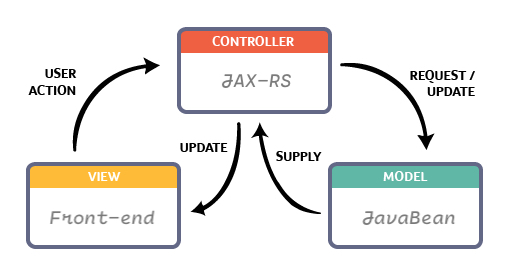
\includegraphics[width=0.9\textwidth]{mvc.jpg}
\caption{\label{fig:mvc}MVC Pattern Applied in this Project}
\end{figure}

Boardly speaking, MovieLobby adopts MVC pattern in system design. Specifically, it is a frontend-backend-seperated project, which uses frameworks in both front-end and back-end, and the two endpoints communicate using web services API, see in [Figure \ref{fig:mvc}].

Hence, in aspect of Model-View-Controller, for this project, Model and Controller are implemented as back-end API server, and View is implemented as front-end web application. 

\newpage
\section{Key Technical Design}

MovieLobby is designed using Vue 3 as front-end framework, and JAX.RS as back-end services. The API is designed in RESTful standard. Besides, MovieLobby adopts IMDb API from RapidAPI (freemium plan) to fetch movie meta data when administrator adding a movie.

In this section, detailed technical implementation will be introduced in three parts, namely front-end, back-end and APIs. Besides, code snippets and running results are provided as follow.

\subsection{Front-end}

\textbf{Adopted tech stack: Vue 3, VueX, Router, Vue SPA Dev, TailwindCSS, Vite.}
\newline

The term front-end has been replaced its usage not only limited in web design nowadays. Modern web application development tools function like traditional JS, HTML, and CSS, however; since node.js, many frameworks have emerged. These frameworks are designed to achieve a higher level of web software design by encapsulating traditional tech stack, especially for JS. I have drawn a diagram [Figure \ref{fig:techs}] that could aid in illustrating the relationship between front-end tech stacks. \cite{aspires}

\begin{figure}[!htp]
\centering
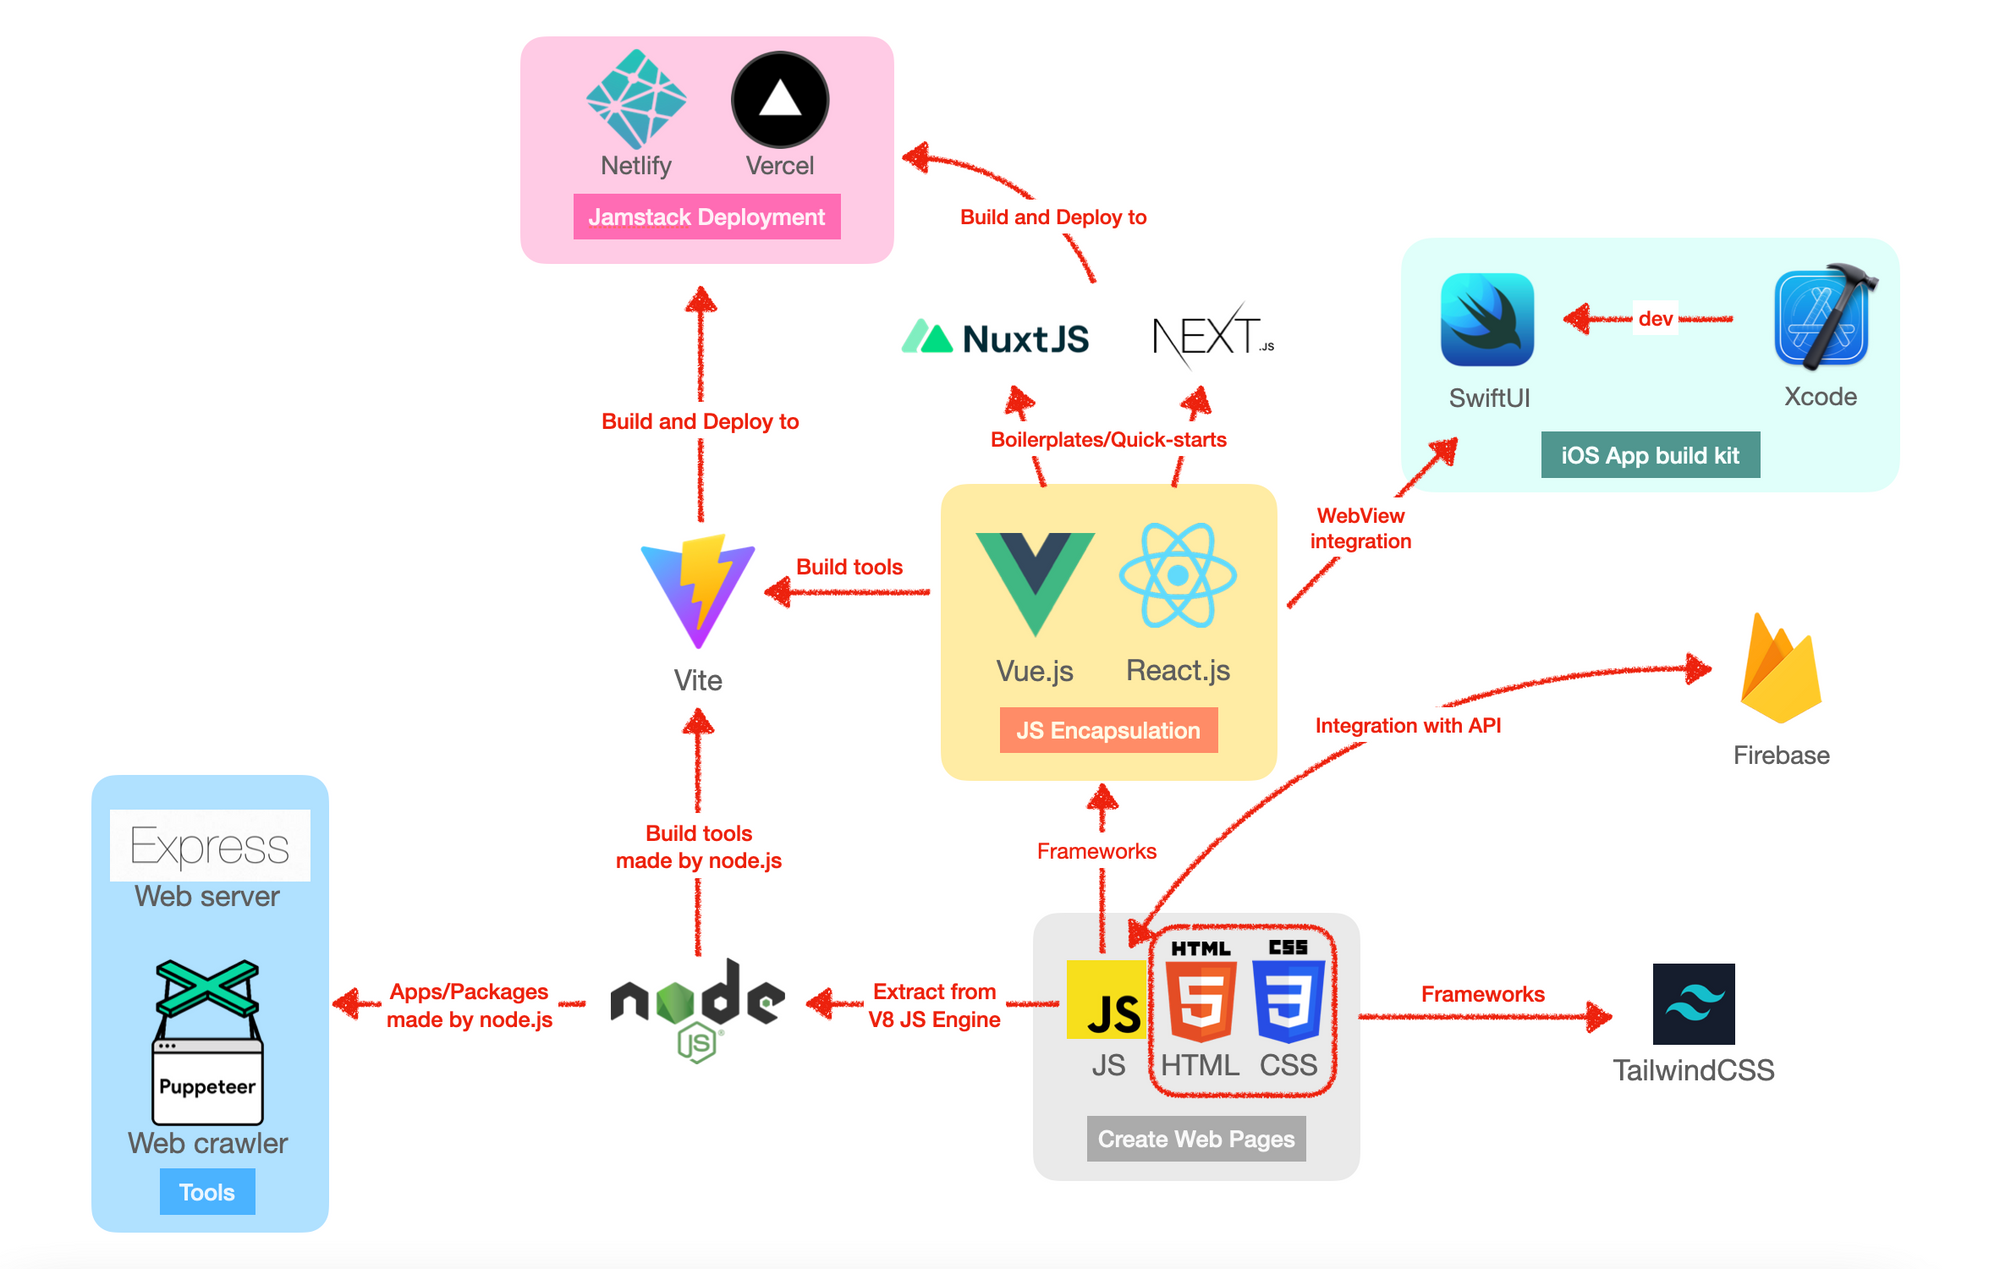
\includegraphics[width=0.9\textwidth]{techs-1.png}
\caption{\label{fig:techs}Front-end tech stacks.}
\end{figure}

\subsubsection{Vue.js Framework}

Vue.js is a progressive framework for building the user interface, which encapsulates DOM and exposes a virtual layer for developers to manipulate with actual DOM in the HTML file. As a result, Vue.js achieve efficient development compared with pure JavaScript. Vue.js 3 is adopted in th front-end project with essential dependencies [Listing \ref{listing:dependencies}]
\begin{listing}[!htp]
\begin{minted}{json}
"dependencies": {
    "autoprefixer": "^10.4.2",
    "postcss": "^8.4.5",
    "tailwindcss": "^3.0.15",
    "vue": "^3.2.25",
    "vue-router": "^4.0.12",
    "vuex": "^4.0.2"
}
\end{minted}
\caption{Dependencies}
\label{listing:dependencies}
\end{listing}

\subsubsection{Vue Single Page Application and Router}

In order to construct front-end web pages as a Single Page Application (SPA). The front-end project adopted vue-router to control the current view to be displayed. Sample router code is shown in [Listing \ref{listing:vue-router}]. In the main entry of front-end Vue 3 project \verb|App.vue|, the router is rendered by vue-router \verb|<router-view/>| tag.

\begin{listing}[!htp]
\begin{minted}{javascript}
import { createRouter, createWebHashHistory, Router } from "vue-router"
import Home from "../views/Home.vue";

const webHistory = createWebHashHistory()

export default createRouter({
  history: webHistory,
  routes: [
    { path: "/", component: Home },
    { path: "/library", component: () => import("../views/Library.vue") },
    { path: "/add/:id", component: () => import("../views/AddMovieConfirm.vue") },
    { path: "/edit/:id", component: () => import("../views/EditMovieConfirm.vue") },
    { path: "/update", component: () => import("../views/AddMovie.vue") },
    { path: "/login", component: () => import("../views/UserLogin.vue") },
    { path: "/rental", component: () => import("../views/Rental.vue") },
  ]
})
\end{minted}
\caption{Vue router}
\label{listing:vue-router}
\end{listing}

\subsubsection{Vite}

Vite is a build tool which allows developers to set up a development environment for frameworks like Vue, and React and even for vanilla JavaScript app with a dev server. \cite{vite} This project is created based on \href{https://github.com/Ex10si0n/quick-starts}{Ex10si0n/quick-starts} template which uses Vite Vue.js template and manually adding the essential dependencies via \verb|yarn| package manager.

To clone the boilerplate GitHub repository, install dependencies and run development server for the front-end project, the following commands are used.

\begin{listing}[!htp]
\begin{minted}{sh}
# clone quick start repo
git clone https://github.com/Ex10si0n/quick-starts.git

# setup local projects
cp -r quick-starts/vue-spa-quick-starts ~/Projects/MovieLobbyWeb
cd ~/Projects/MovieLobbyWeb

# install dependencies and starting development server
yarn
yarn dev
\end{minted}
\caption{Installing dependencies and run development server}
\label{listing:yarn}
\end{listing}


\subsubsection{Tailwind CSS Framework}

Tailwind CSS is basically a utility-first CSS framework for rapidly building custom user interfaces. It is a highly customizable, low-level CSS framework that gives the developer all of the building blocks they need to build bespoke designs without any annoying opinionated styles that have to fight to override. \cite{tw}

Tailwind CSS works well with Vue.js components without coding extra CSS style sheet. The code snippet below [Listing \ref{listing:movie-card}] displays style declaration in movie card component \verb|<MovieCard/>| in our front-end project.

\begin{listing}[!htp]
\begin{minted}{html}
<template>
  <div class="flex flex-col items-center rounded-lg border shadow-md md:flex-row
  border-black bg-black my-4">
    <img class="object-cover w-1/3 rounded-l-lg" :src="coverImage" alt="">
    <div class="flex flex-col justify-between p-4 leading-normal">
      <div class="flex flex-col space-y-4">
        <div class="flex justify-between items-start">
          <h2 class="text-3xl font-bold">{{ title }}</h2>
        </div>
        <div class="text-sm text-gray-400">{{ genre }}</div>
        <div class="text-lg text-gray-200">{{ year }}</div>
        <div class="text-gray-400 max-h-40 overflow-y-hidden">{{ description }}</div>
        <div class="flex text-2xl font-bold text-a">${{ rentalPrice }}</div>
      </div>
      <div class="grid grid-cols-2">
        <button class="mt-12 text-black bg-white rounded-lg px-4 py-2 font-bold
        w-28 col-span-1" @click="rent">Rent</button>
        <button class="mt-12 text-blue-600 rounded-lg px-4 py-2 font-bold w-28
        col-span-1" @click="edit">Edit</button>
      </div>
    </div>
  </div>
</template>
\end{minted}
\caption{Using tailwind CSS in Vue component}
\label{listing:movie-card}
\end{listing}

\subsection{Back-end}
\textbf{Adopted tech stack: JAX.RS, Jakarta.Persistence (JPA), Gson, Glassfish, MariaDB}

The back-end part of this project is designed as an API services application server, which including a database, and Jakarta EE RESTful API server JAX.RS. The database connection is implemented with technique of JPA, specifically; it contains Jakarta Persistence API with MaraiaDB JDBC connector API.


\subsubsection{MariaDB deployment}

MariaDB is one of the most popular open-source relational database management system and could be used as a great replacement of MySQL. It is developed by original developers of MySQL. MariaDB can also stores data in various tables. It is also part of most cloud offerings and default in most Linux distributions. \cite{mariadb}

Docker is a software platform that allows developers to build, test, and deploy applications quickly. Docker packages software into standardized units called containers that have everything the software needs to run including libraries, system tools, code, and runtime. Using Docker, developers can quickly deploy and scale applications into any environment.
\cite{docker}

In the project, the database management system is MariaDB, and it is deployed with Docker. The deployment command is [Listing \ref{listing:docker}]. Docker MariaDB container expose port 3306 and mapping to the port 3306 of the host machine.

\begin{listing}[!htp]
\begin{minted}{sh}
$ docker run --name eis-mdb
    \ -e MYSQL_ROOT_PASSWORD=******
    \ -p 3306:3306 -d mariadb
\end{minted}
\caption{Deploy MariaDB using Docker}
\label{listing:docker}
\end{listing}

To test the connection of database in docker, we could use Tableplus. The test connection interface is shown in [Figure \ref{fig:tableplus}].

\begin{figure}[!htp]
\centering
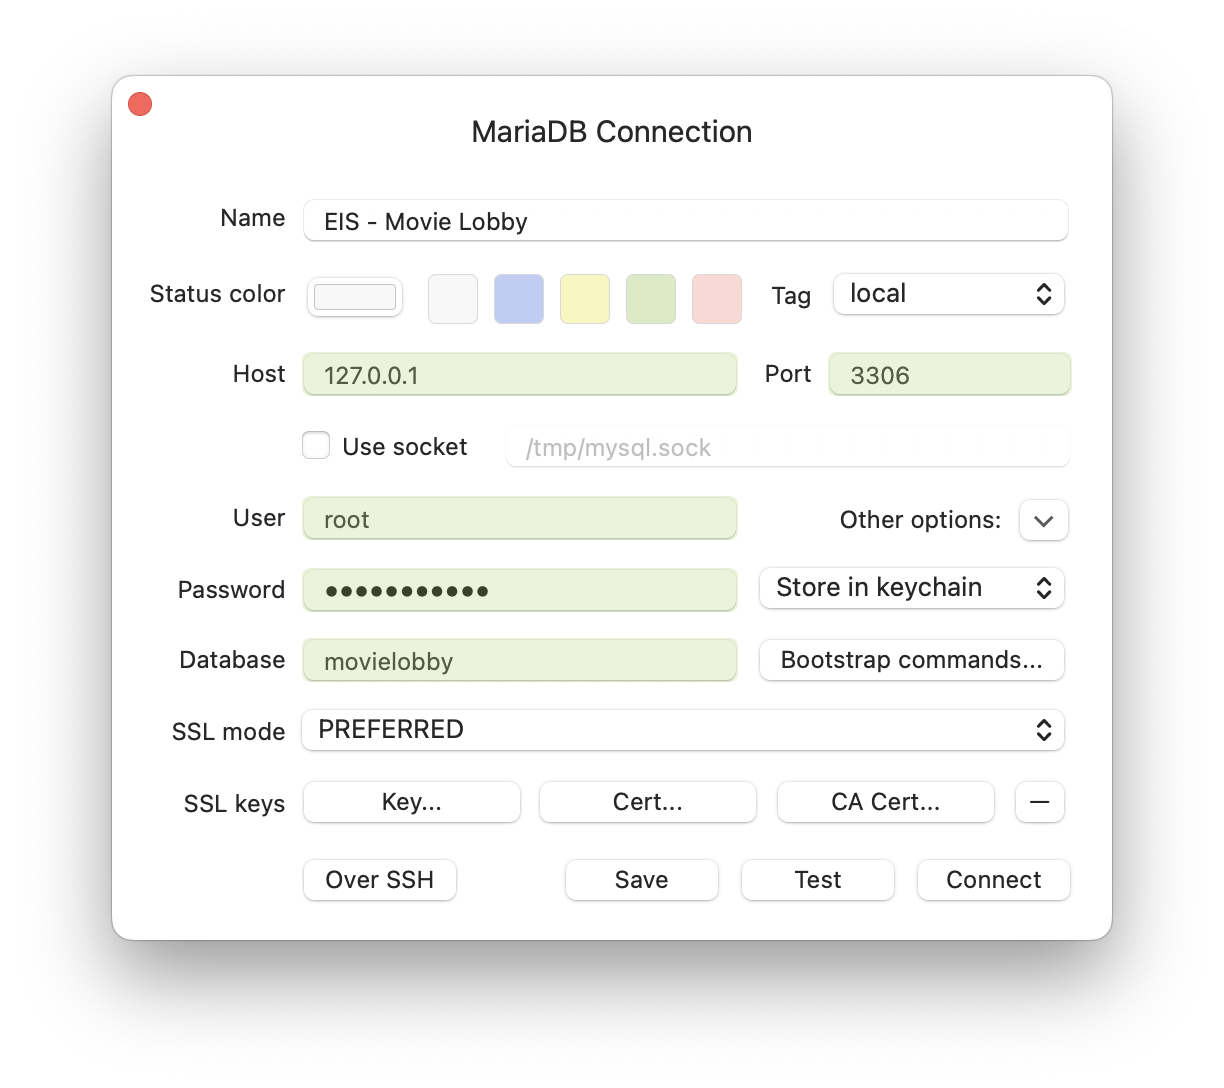
\includegraphics[width=0.65\textwidth]{tableplus.png}
\caption{\label{fig:tableplus}Tableplus database tool}
\end{figure}

\subsubsection{Dependencies}

This project uses Maven as a package manager. Essential dependencies are described in the following list [Listing \ref{listing:dep}] according to \verb|pom.xml|.

\begin{listing}[!htp]
\begin{minted}{xml}
<dependency>
    <groupId>jakarta.ejb</groupId>
    <artifactId>jakarta.ejb-api</artifactId>
    <version>4.0.0</version>
    <scope>provided</scope>
</dependency>
<dependency>
    <groupId>jakarta.ws.rs</groupId>
    <artifactId>jakarta.ws.rs-api</artifactId>
    <version>3.0.0</version>
    <scope>provided</scope>
</dependency>
<dependency>
    <groupId>org.hibernate.orm</groupId>
    <artifactId>hibernate-core</artifactId>
    <version>6.0.0.Final</version>
</dependency>
<dependency>
    <groupId>org.mariadb.jdbc</groupId>
    <artifactId>mariadb-java-client</artifactId>
    <version>LATEST</version>
</dependency>
<dependency>
    <groupId>com.google.code.gson</groupId>
    <artifactId>gson</artifactId>
    <version>2.2.2</version>
    <scope>compile</scope>
</dependency>
\end{minted}
\caption{Dependencies}
\label{listing:dep}
\end{listing}


\subsubsection{Database Definition using ORM}

To construct the structure of relational database, we usually use data definition language (DDL). However, in this project, with adopting object–relational mapping (ORM) implemented with JPA, DDL could be omit and its function is replaced by definitions in Java Bean for each entity. For example, the following code snippet [Listing \ref{listing:moviebean}] shows attributes of MovieBean and their mapping definitions.

\begin{listing}[!htp]
\begin{minted}{java}
package cc.aspires.movielobby.model;

import jakarta.persistence.Column;
import jakarta.persistence.Entity;
import jakarta.persistence.Id;
import jakarta.persistence.Table;

@Entity
@Table(name = "Movie")
public class Movie {
    @Id
    @Column(name = "id")
    private String id;

    @Column(name = "title")
    private String title;

    // More attributes omitted ...

    public void setId(String id) { this.id = id; }

    public String getId() { return id; }

    // Getters and setters are omitted ...
}
\end{minted}
\caption{MovieBean}
\label{listing:moviebean}
\end{listing}

To create tables, we could create a \verb|MovieModel| class and directly use entity manager to persist data into database. See [Listing \ref{listing:moviemodel}]. By invoking \verb|addMovie()| method, the Movie table is created automatically into the database. For initiating the database at first time run, the code is provided at package: \verb|cc.aspires.movielobby.test|.

\begin{listing}[!htp]
\begin{minted}{java}
public static String addMovie(Movie movie) {
    EntityManagerFactory entityManagerFactory = 
        Persistence.createEntityManagerFactory("default");
    EntityManager entityManager = entityManagerFactory.createEntityManager();
    String res;
    try {
        entityManager.getTransaction().begin();
        entityManager.persist(movie);
        entityManager.getTransaction().commit();
        res = "success";
    } catch (Exception e) {
        res = "failed";
    }
    entityManager.close();
    entityManagerFactory.close();
    return res;
}
\end{minted}
\caption{Movie Model}
\label{listing:moviemodel}
\end{listing}

\subsubsection{JAX-RS RESTful Web Service API Server}

JAX-RS is a Java based programming language API and specification to provide support for created RESTful web services \cite{jaxrs}. An example of implementation a web service that provides GET and POST handling for movie resources is shown in [Listing \ref{listing:movieresources}].

\begin{listing}[!htp]
\begin{minted}{java}
package cc.aspires.movielobby.resources;

import cc.aspires.movielobby.model.MovieModel;
import cc.aspires.movielobby.model.Movie;
import com.google.gson.Gson;
import jakarta.ws.rs.*;

@Path("/movie")
public class MovieResource {

    @POST
    @Consumes("application/json")
    @Produces("application/json")
    @Path("/add")
    public String addMovie(Movie movie) {
        String response = MovieModel.addMovie(movie);
        return "{\"response\": " + response + "}";
    }
    // more methods omitted ...
}
\end{minted}
\caption{Movie Resources}
\label{listing:movieresources}
\end{listing}

\verb|@Path| annotation helps to standardize the API request URL in RESTful style. For example, the presented code snippets created a API endpoint with URL \verb|/api/movie/add| for handling `POSTed' JSON object. The \verb|MovieResouce| calls \verb|addMovie| method inside \verb|MovieModel| class to conducting the business logic for persisting movie data.

\subsection{APIs}

The term API refers two components in this project. Specifically, data communication between front-end and back-end, and the movie meta data fetching process from IMDb. 

\subsubsection{Back-end Service API}

This project implemented a back-end API server to commit data communication follow the standard of RESTful. JAX-RS is configured in \verb|APIServiceConfiguration| class simply using the following code [Listing \ref{listing:config}]. Moreover, configured API URLs are listed in the following list [Listing \ref{listing:apiurl}].

\begin{listing}[!htp]
\begin{minted}{java}
package cc.aspires.movielobby.services;

import jakarta.ws.rs.ApplicationPath;
import jakarta.ws.rs.core.Application;

@ApplicationPath("/api")
public class APIServiceConfiguration extends Application { 
    
}
\end{minted}
\caption{Service Configuration}
\label{listing:config}
\end{listing}

\begin{listing}[!htp]
\begin{minted}{sh}
# Movie Resources
/api/movie/all GET
/api/movie/get/{id} GET
/api/movie/add POST
/api/movie/update POST
/api/movie/delete POST

# Rental Resources
/api/rental/rent/{movieId}/{email} GET
/api/rental/get/{email} GET

# User Resources
/api/user/login POST
/api/user/signup POST
/api/user/token/{email} GET
/api/user/token/topup/{email}/{value} GET
\end{minted}
\caption{API Endpoints}
\label{listing:apiurl}
\end{listing}

Curl is a command-line (CLI) tool for transferring data specified with URL syntax. It could send POST request using CLI. For example, the screenshot [Figure \ref{fig:curl}] below shows the way of adding a movie (in JSON) into the database.

\begin{figure}[!htp]
\centering
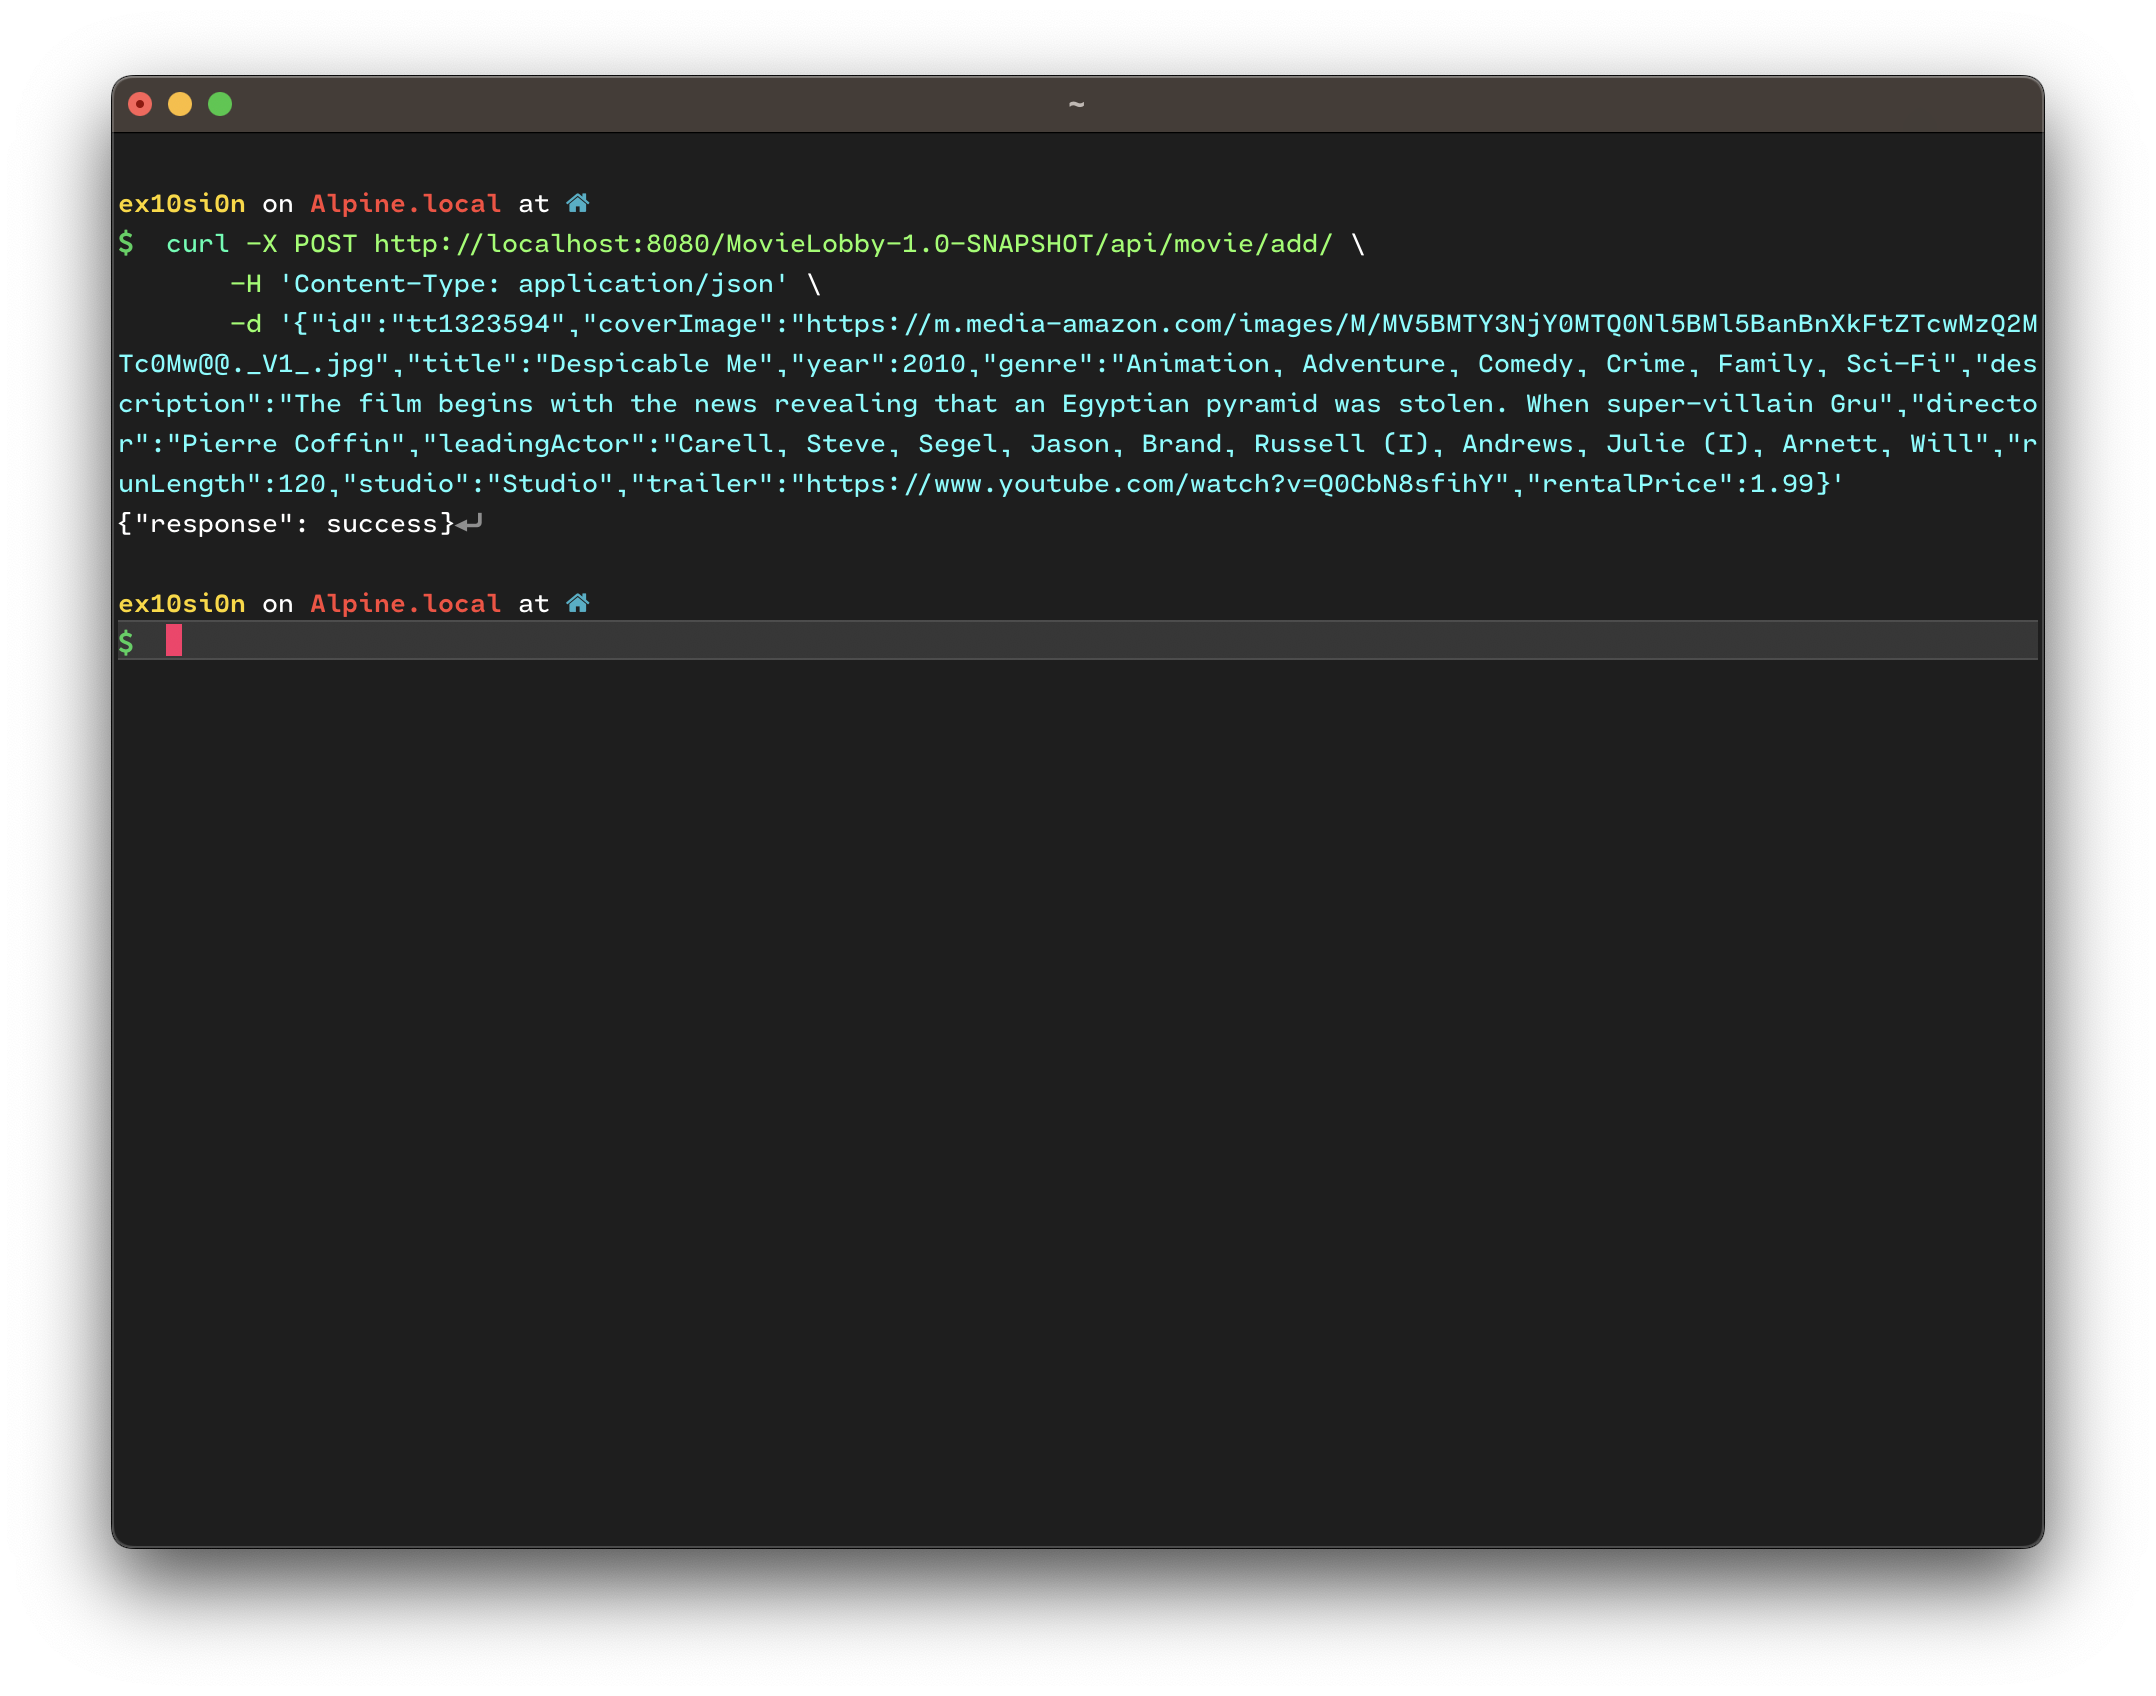
\includegraphics[width=1\textwidth]{curl.png}
\caption{\label{fig:curl}cURL send POST request}
\end{figure}

\subsubsection{IMDb API}

This project adopted IMDb API from RapidAPI (freemium usage) for fetching meta data of movies. The API is called in front-end side, mainly in adding movies function. The code of calling IMDb API for fuzzy searching is shown in [Listing \ref{listing:fuzzy}], 

\begin{listing}[!htp]
\begin{minted}{javascript}
const searchMovie = () => {
  // clear search results
  searchResults.splice(0, searchResults.length)
  const url = 'https://imdb8.p.rapidapi.com/auto-complete/' +
    '?q=' + searchTitle.value;

  const options = {
    method: 'GET',
    headers: {
      'X-RapidAPI-Key': api.imdb.key,
      'X-RapidAPI-Host': 'imdb8.p.rapidapi.com'
    },
  };

  fetch(url, options)
    .then(res => res.text())
    .then(json => {
      JSON.parse(json).d.forEach(movie => {
      if (movie.i && movie.id && movie.l && movie.q && movie.y && movie.s) {
        searchResults.push(movie)
      }
    })
  })
}
\end{minted}
\caption{Calling IMDb fuzzy searching API}
\label{listing:fuzzy}
\end{listing}

\section{Entity Relationship}
Entity Relation (ER) Diagram is shown in [Figure \ref{fig:er}], generated by Intellij IDEA based on Java Bean.

\begin{figure}[!htp]
\centering
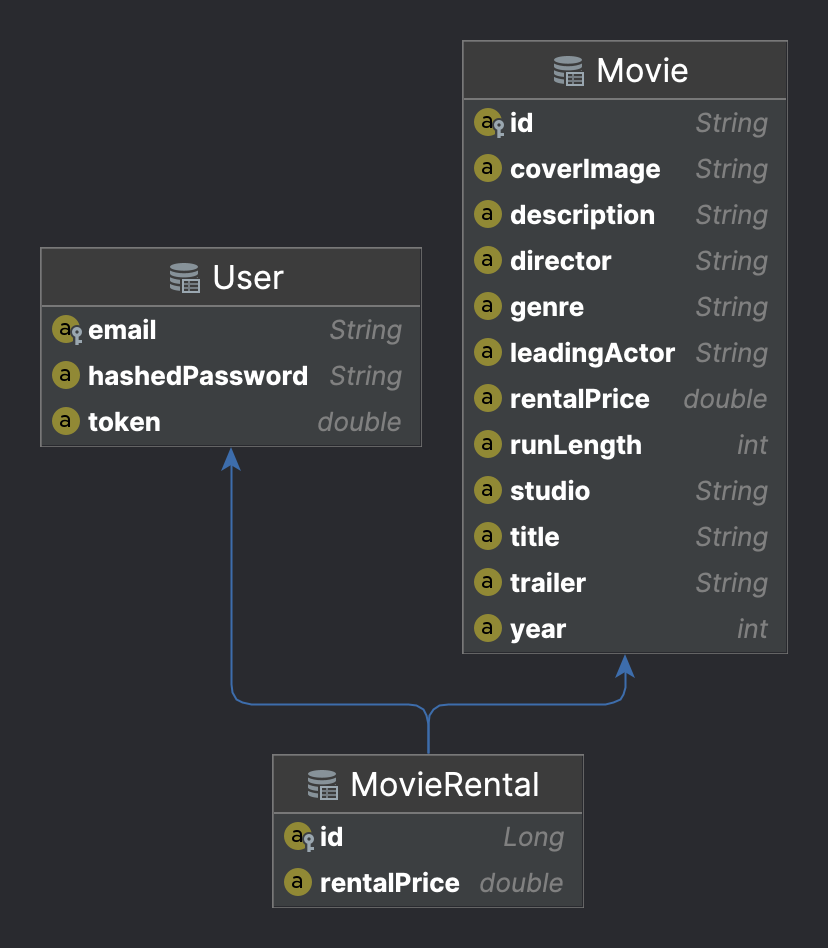
\includegraphics[width=0.4\textwidth]{er.png}
\caption{\label{fig:er}ER Diagram}
\end{figure}

\section{Class Diagrams}

Class Diagram is shown in [Figure \ref{fig:cls}]

\begin{figure}[!htp]
\centering
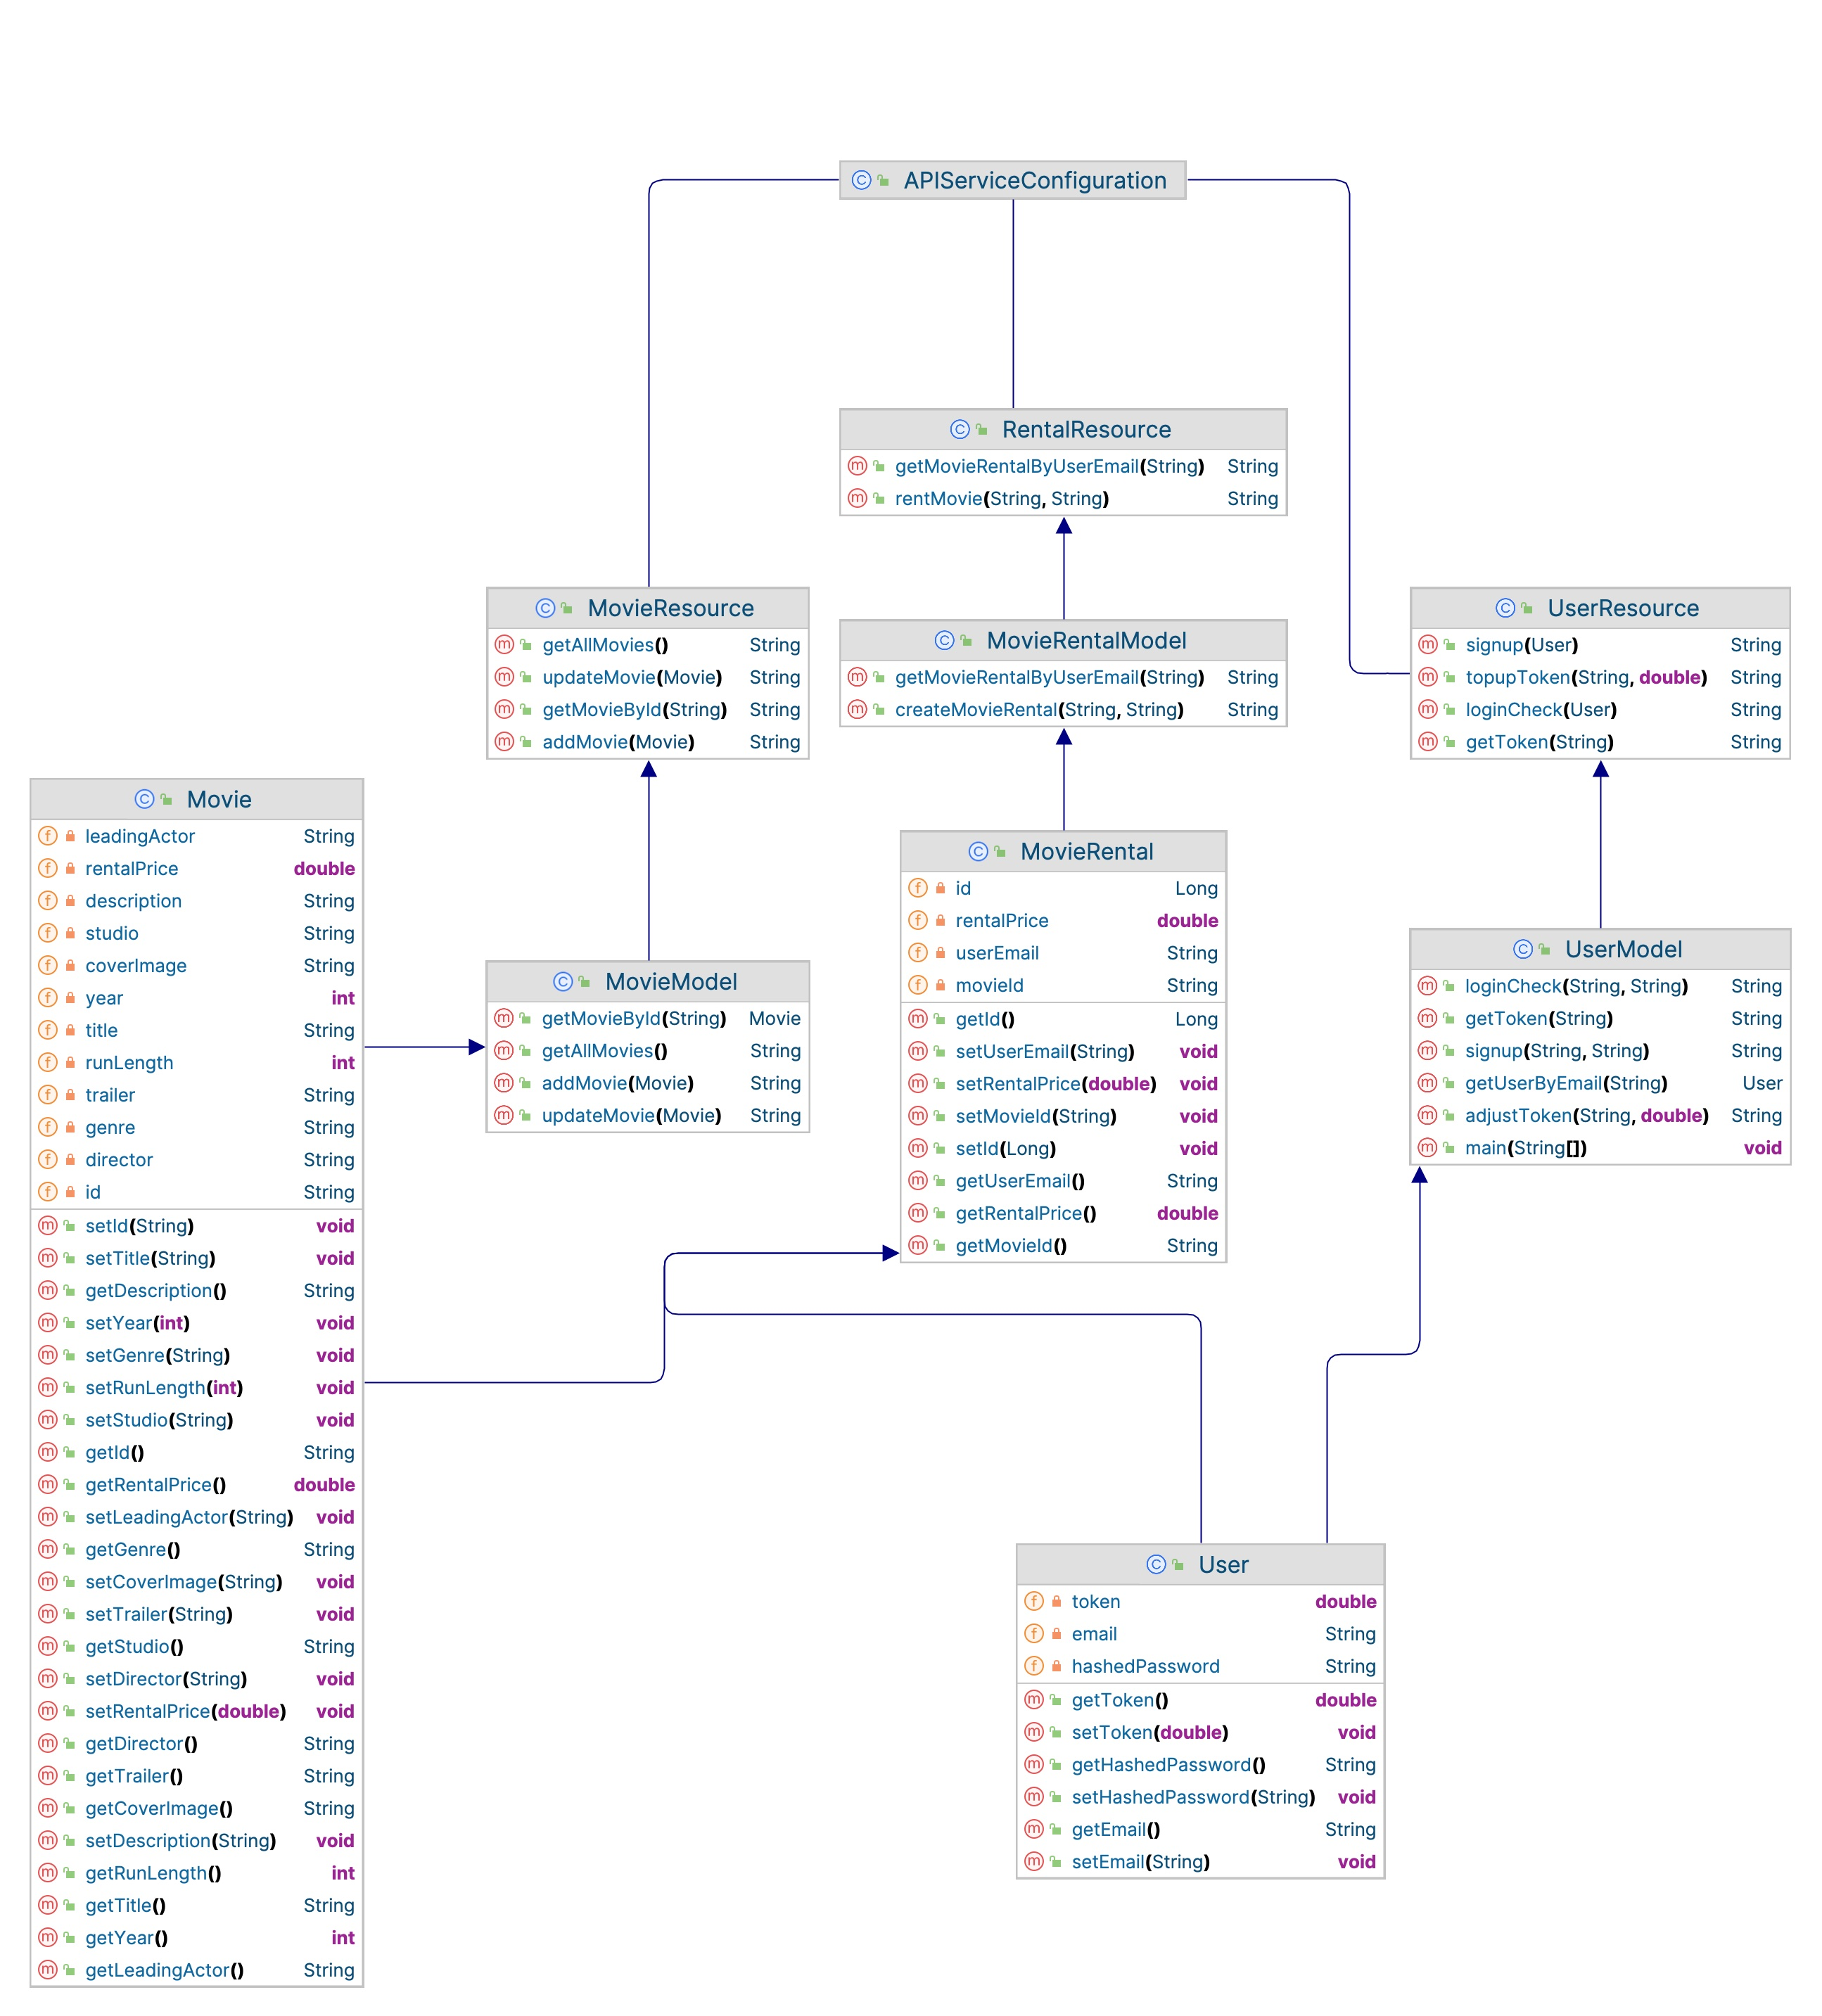
\includegraphics[width=1\textwidth]{class.jpg}
\caption{\label{fig:cls}Class Diagram}
\end{figure}

\section{Sitemapping}

Sitemap diagram is shown as follow in [Figure \ref{fig:sitemap}]

\begin{figure}[!htp]
\centering
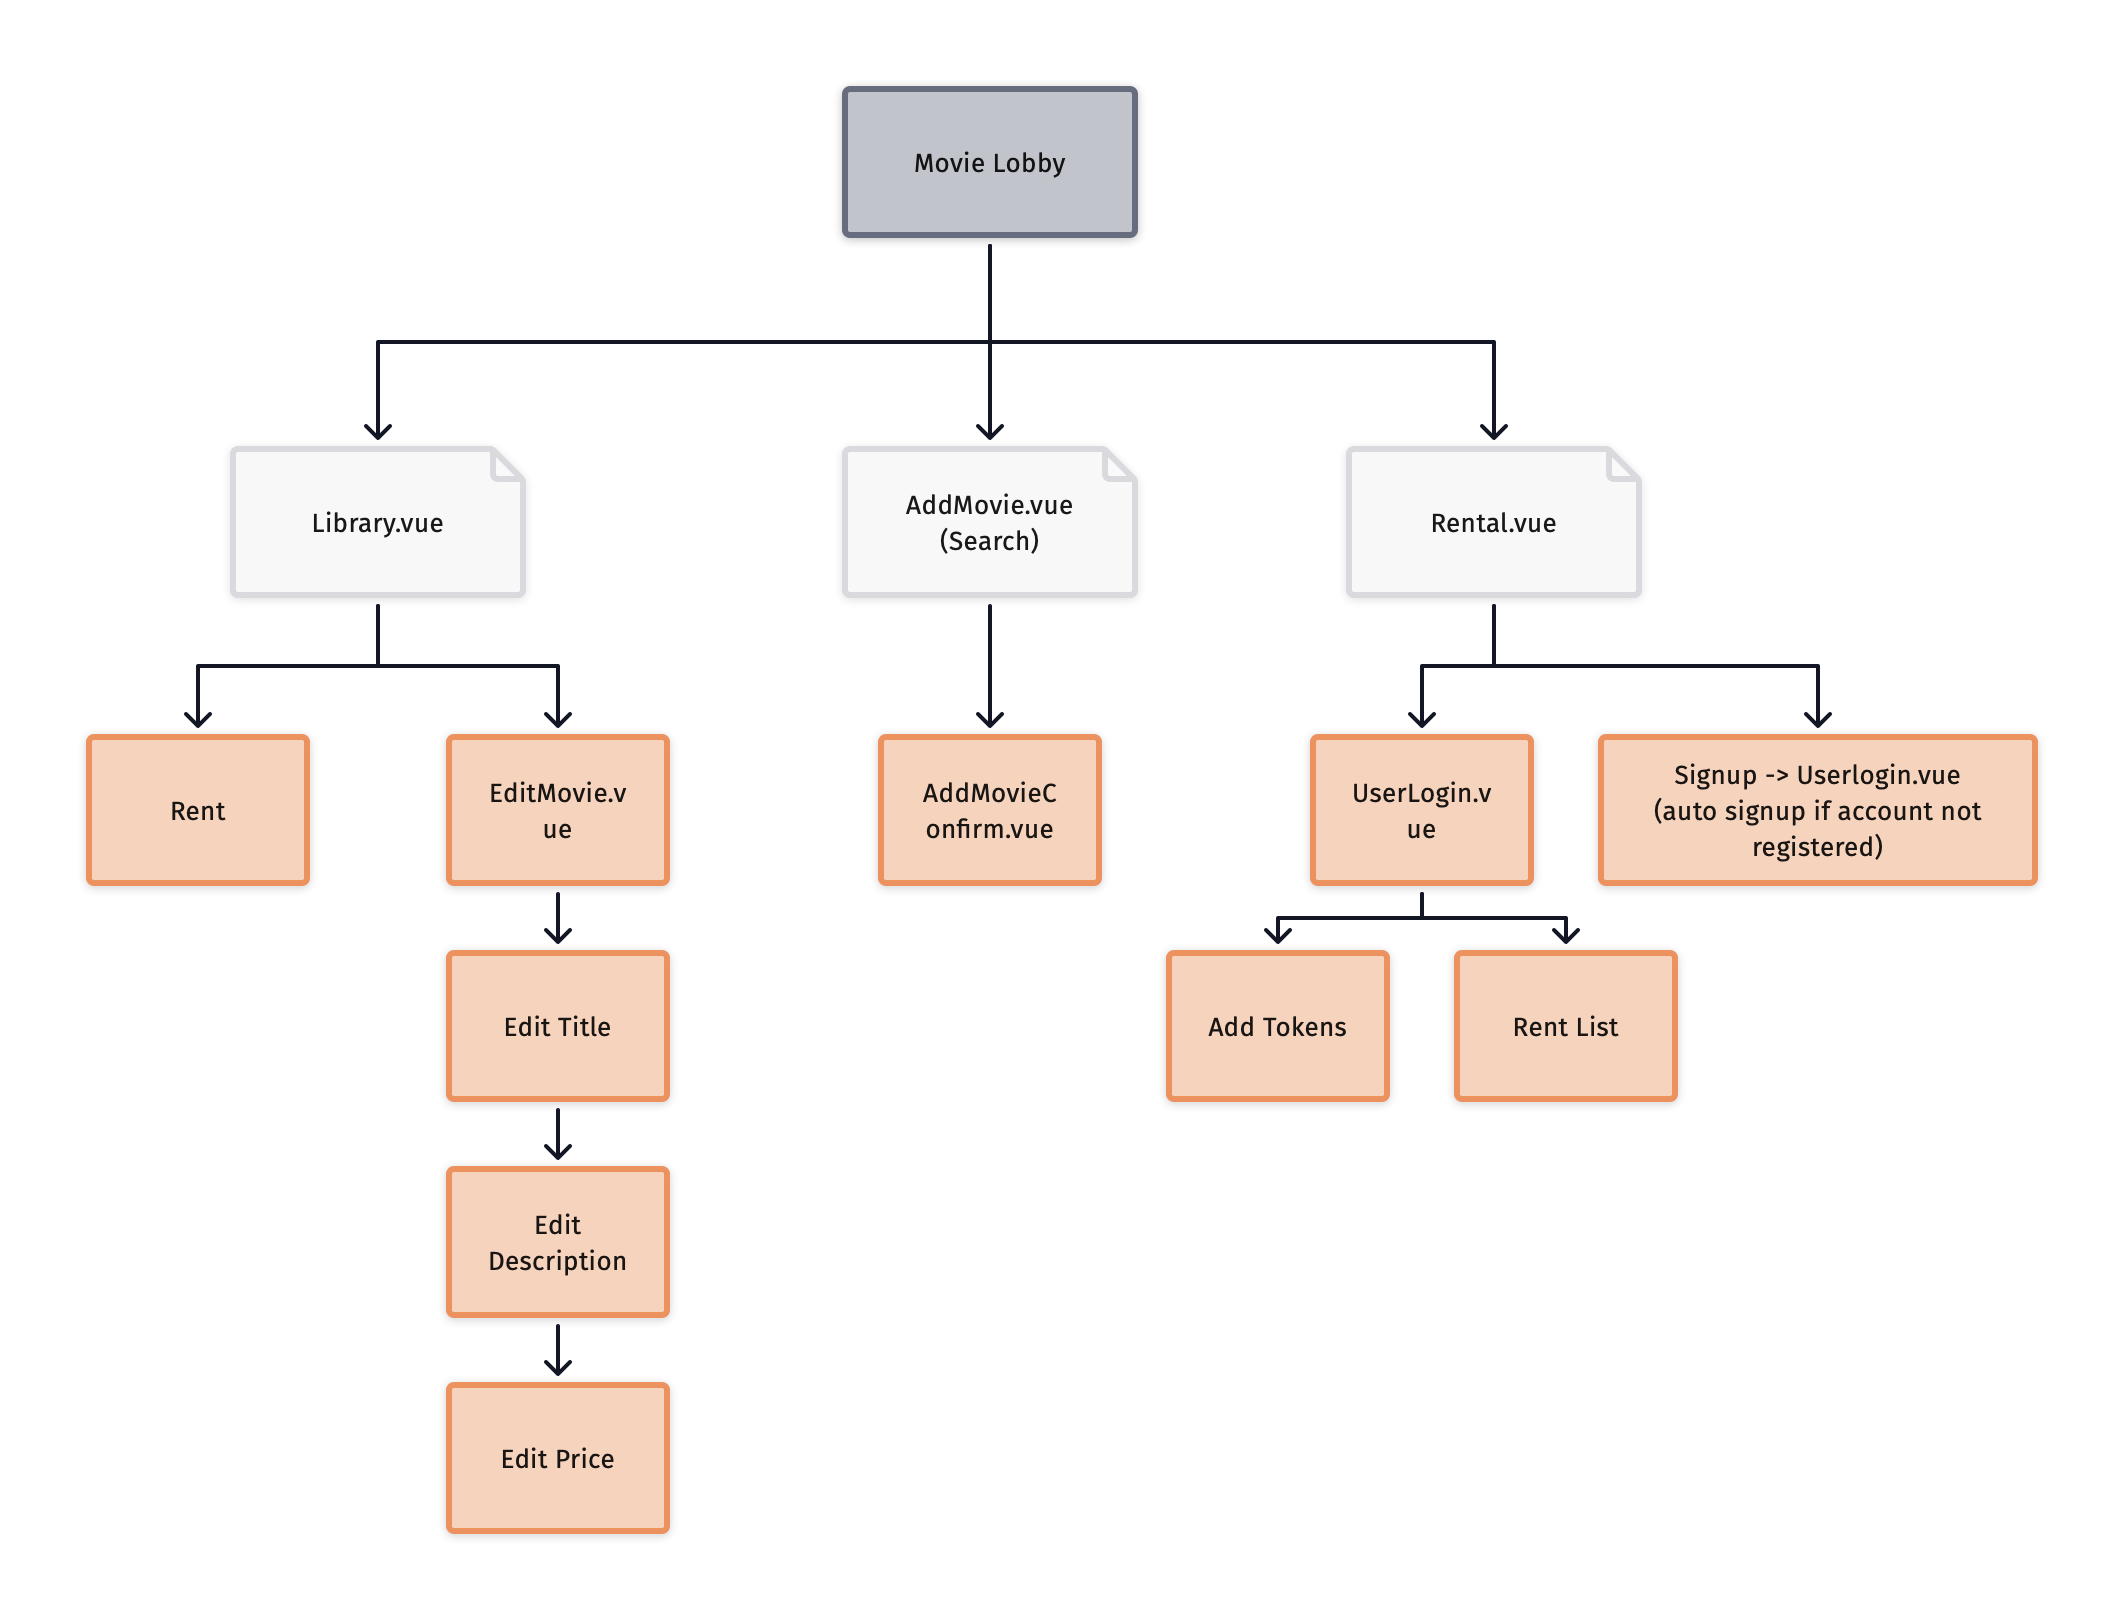
\includegraphics[width=1\textwidth]{sitemap.png}
\caption{\label{fig:sitemap}Sitemap Diagram}
\end{figure}

\section{User Interface}

In this section, application UI screenshot will be presented as follow. Specifically, user login and signup in [Figure \ref{fig:login}], search moive in [Figure \ref{fig:search}], add movie in [Figure \ref{fig:add}], and edit movie in [Figure \ref{fig:edit}].

\begin{figure}[!htp]
\centering
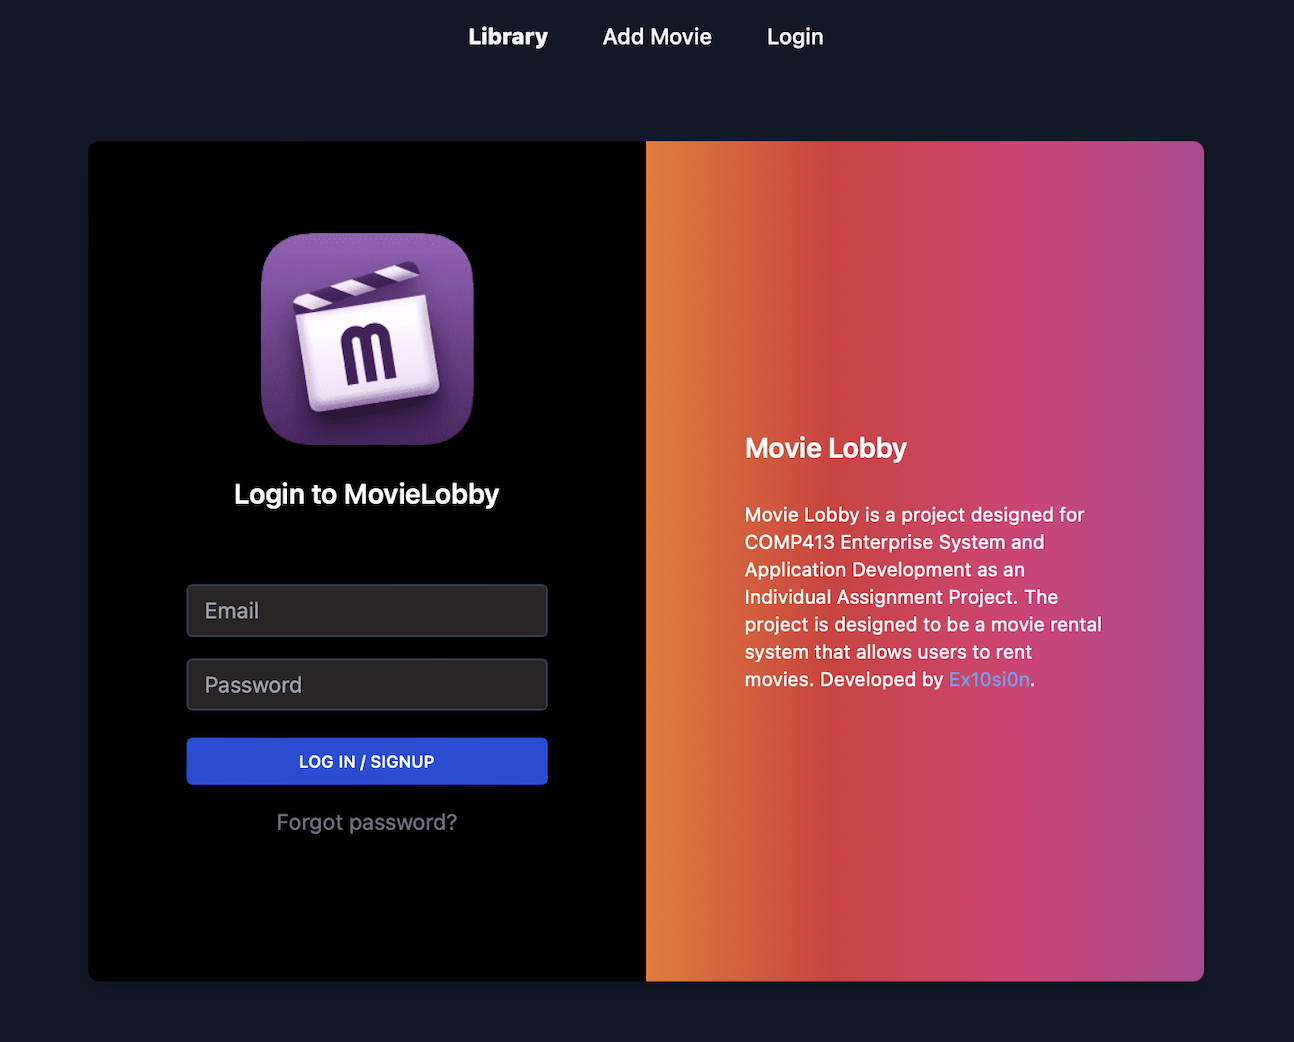
\includegraphics[width=0.7\textwidth]{login.png}
\caption{\label{fig:login}Login and Signup}
\end{figure}

\begin{figure}[!htp]
\centering
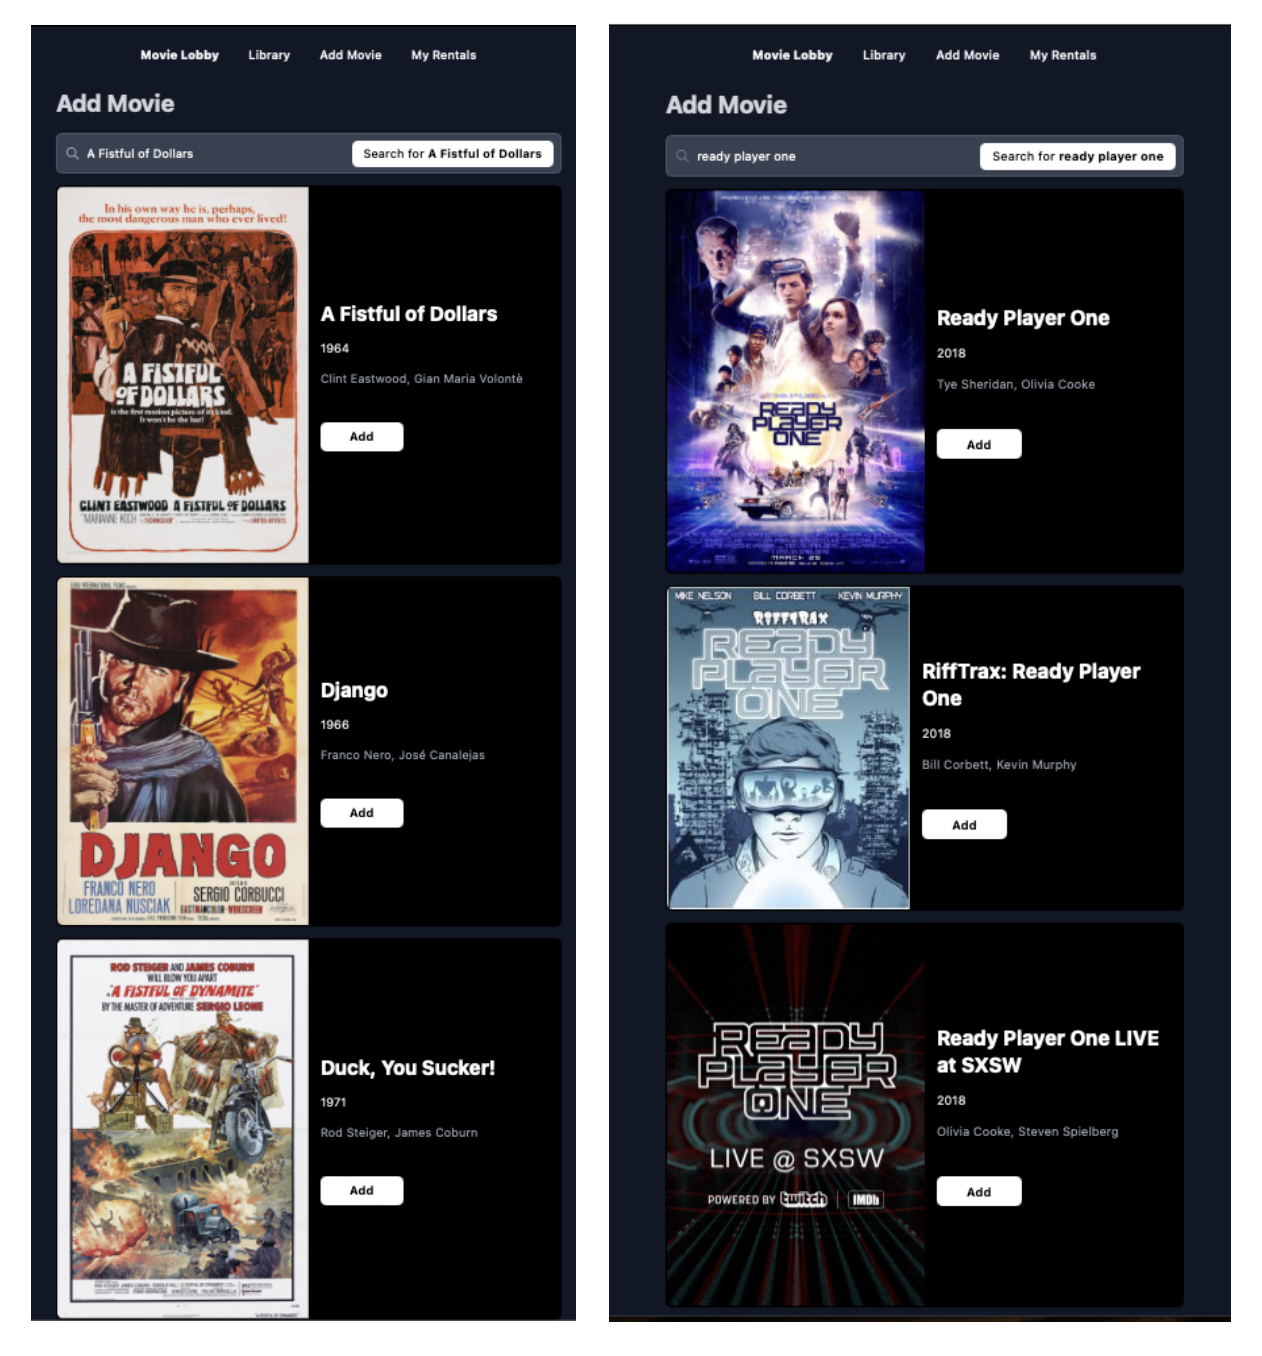
\includegraphics[width=0.7\textwidth]{search.png}
\caption{\label{fig:search}Search Movie}
\end{figure}

\begin{figure}[!htp]
\centering
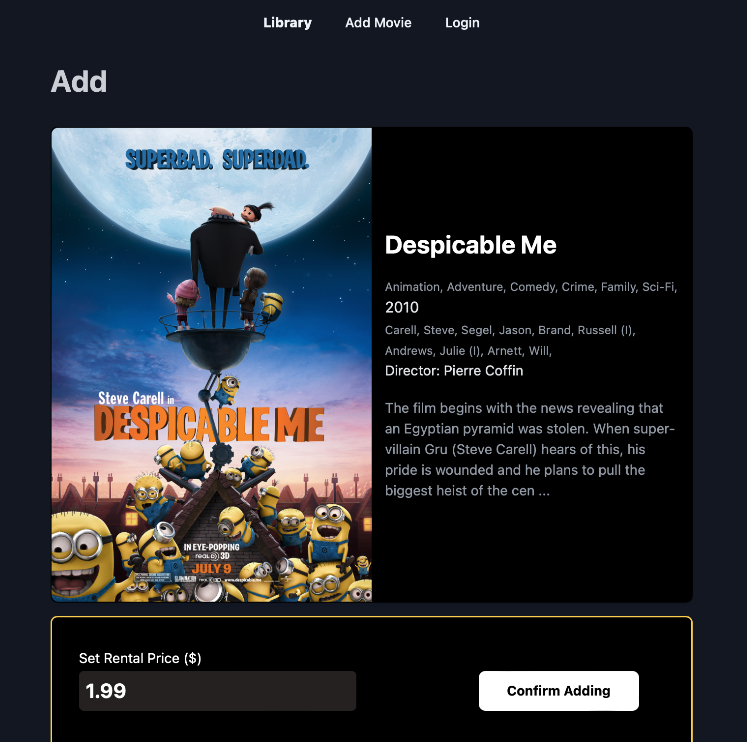
\includegraphics[width=0.7\textwidth]{add.png}
\caption{\label{fig:add}Add Movie}
\end{figure}

\begin{figure}[!htp]
\centering
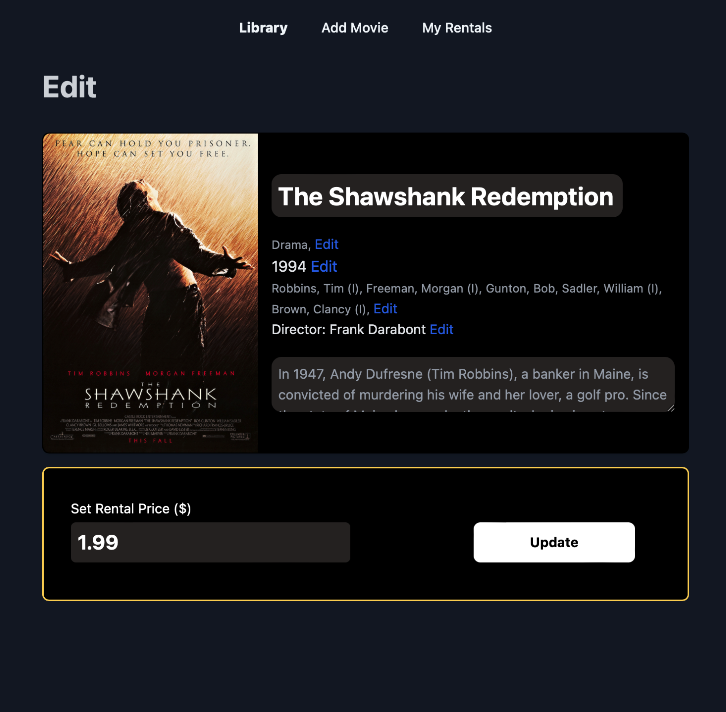
\includegraphics[width=0.7\textwidth]{edit.png}
\caption{\label{fig:edit}Edit Movie}
\end{figure}

\newpage
\bibliographystyle{ieeetr}
\bibliography{sample}

\end{document}